\documentclass[9pt,twocolumn,twoside]{pnas-new}
% Use the lineno option to display guide line numbers if required.
% Note that the use of elements such as single-column equations
% may affect the guide line number alignment.

\templatetype{pnasresearcharticle} % Choose template
% {pnasresearcharticle} = Template for a two-column research article
% {pnasmathematics} = Template for a one-column mathematics article
% {pnasinvited} = Template for a PNAS invited submission

% added to enable supplementary figures
\usepackage{placeins}
\usepackage{newfloat}
\usepackage{xr-hyper}
\externaldocument{manuscript_noSI}
\DeclareFloatingEnvironment[name={Figure}]{suppfigure}
\renewcommand{\thesuppfigure}{S\arabic{suppfigure}}

\DeclareFloatingEnvironment[name={Dataset}]{suppdata}
\renewcommand{\thesuppdata}{S\arabic{suppdata}}

\setcounter{topnumber}{10}
\setcounter{bottomnumber}{10}
\setcounter{totalnumber}{10}

\newcommand{\comment}[1]{{\color{red}[\textsl{#1}]}}


\begin{document}

% Please give the surname of the lead author for the running footer
\leadauthor{Lee}

\dates{This manuscript was compiled on \today}
\doi{\url{www.pnas.org/cgi/doi/10.1073/pnas.XXXXXXXXXX}}


% Optional adjustment to line up main text (after abstract) of first page with line numbers, when using both lineno and twocolumn options.
% You should only change this length when you've finalised the article contents.
\verticaladjustment{-2pt}

\onecolumn

\clearpage
\section*{Supporting Information (SI)}
\FloatBarrier
\pagenumbering{arabic}% resets `page` counter to 1
\renewcommand*{\thepage}{S\arabic{page}}

\begin{suppfigure}[H]
\centerline{\includegraphics[width=0.5\textwidth]{figs/supp_G78D-T212I/G78D-T212I.pdf}}
\caption{\label{suppfig:Perth2009_mut}
{\bf Characterization of the G78D-T212I Perth/2009 HA variant.}
(A)
The G78D-T212I Perth/2009 HA variant supports better viral growth than the wildtype Perth/2009 HA.
Viruses were generated in duplicate by reverse genetics with the Perth/2009 NA and WSN internal genes, and passaged once at MOI = 0.01 in MDCK-SIAT1-TMPRSS2 cells.
The rescue and passage viral supernatants were collected at 72 hours post-transfection and 44 hours post-infection, respectively, and titered in MDCK-SIAT1-TMPRSS2 cells.
The points mark each duplicate and the bar marks the mean.
(B)
The D78 variant remained at a low frequency in natural human H3N2 sequences over the past $~\sim$10 years.
The A212 variant rose to fixation in $~\sim$2011, replacing the T212 variant.
}
\end{suppfigure}

\begin{suppfigure}[H]
\centerline{
\includegraphics[width=0.6\textwidth]{figs/supp_SangerSeq/SangerSeq.pdf}}
\caption{\label{suppfig:SangerSeq}
{\bf Sanger sequencing of 31 randomly chosen clones from the mutant plasmid libraries.}
(A) There were an average of $\sim$1.4 codon mutations per clone across the three plasmid mutant libraries.
(B) A mixture of one-, two-, and three-nucleotide mutations were present, with slightly fewer triple-nucleotide changes than expected.
(C) Nucleotide frequencies were uniform in the codon mutations.
(D) The mutations were distributed relatively evenly across the length of the HA coding sequence.
(E) We calculated the pairwise distances between mutations for clones carrying more than one mutation.
The cumulative distribution of these distances is shown in the red line.
The blue line indicates the expected distribution if mutations in multiply mutated genes are randomly dispersed along the sequence.
}
\end{suppfigure}

\begin{suppfigure}[H]
\centerline{\includegraphics[width=0.9\textwidth]{figs/supp_diffprefs/diffprefs.pdf}}
\caption{\label{suppfig:diffprefs_logoplot}
{\bf Sites where there are strong differences between our experimental measurements and the amino-acid frequencies among natural HA sequences.}
We calculated the distance between our H3 measurements and the alignment frequencies using the same approach as in Figure~\ref{fig:distance_distribution}, but using the alignment frequencies in place of the H1 preferences.
For each site, the height of each letter above or below the line indicates how much more or less preferred that amino acid is in our experiments compared to its frequency nature.
The overlays show the same information as in Figure~\ref{fig:logoplot} (domain and wildtype amino acid).
The sites are in H3 numbering.
The HA alignment used to calculate the natural frequencies is the same one used in Table~\ref{tab:phydms}.
}
\end{suppfigure}

\begin{suppfigure}[H]
\centerline{\includegraphics[width=0.4\textwidth]{figs/supp_point_mut_validation/startcodon_titers.pdf}}
\caption{
{\bf Validation that the Perth/2009 HA is somewhat tolerant to mutation of the canonical start codon.}
We created variants of the Perth/2009 HA in which the canonical start codon was mutated (amino-acid mutation M(-16)K, codon mutation ATG$\rightarrow$AAA), a conserved cysteine was mutated to alanine (C52A, codon mutation TGC$\rightarrow$GCA), and the same cysteine was synonymously mutated (C52C, codon mutation TGC$\rightarrow$TGT).
We selected these mutations because our deep mutational scanning results in Figure~\ref{fig:logoplot} surprisingly suggest that the start codon (position -16) is fairly tolerant of mutations, but that site 52 is highly intolerant of mutation to anything other than cysteine.
The synonymous C52C mutation is a negative control mutation that is not expected to have any effect.
We then used reverse genetics to generate viruses carrying the wildtype HA or each point mutant, with GFP packaged in the PB1 segment to enable easy titering by flow cytometry~\cite{bloom2010permissive,hooper2013mutant}.
Each variant was generated in duplicate, and the plots show the viral titer in the supernatant at 53 hours post-transfection.
As expected, the C52A virus is essentially non-viable, while the C52C mutation is roughly equivalent to wildtype.
The M(-16)K mutation is only moderately attenuated, validating that the canonical start codon is not completely essential for viral growth.
}
\label{suppfig:startcodon_validation}
\end{suppfigure}

\begin{suppfigure}[H]
\centerline{\includegraphics[width=0.4\textwidth]{figs/supp_point_mut_validation/glycan_titers.pdf}}
\caption{\label{suppfig:glycan_validation}
{\bf Validation of viral variants with mutations at N-linked glycosylation motifs.}
We created variants of the Perth/2009 HA with mutations that eliminated N-linked glycosylation motifs (Asn-Xaa-Ser/Thr) at asparagine residues 22, 38, and 285 (these are mutations T24F, T40V, and S287A, respectively).
The codon mutations were ACG$\rightarrow$TTC, ACT$\rightarrow$GTA, and AGC$\rightarrow$GCG, respectively.
We then used reverse genetics to generate viruses carrying the wildtype HA or each of these mutants.
Each variant was generated in duplicate, and the plots show the viral titer in the supernatant at 53 hours post-transfection.
The viruses with mutations at the motifs at residues 22 and 38 reached titers at least as high as wildtype, whereas the virus with a mutation to the motif at residue 285 was modestly attenuated.
}
\end{suppfigure}

\begin{suppfigure}[H]
\centerline{\includegraphics[width=0.45\textwidth]{figs/supp_point_mut_validation/tm_titers.pdf}}
\caption{\label{suppfig:TM_validation}
{\bf Validation of the mutational tolerance of a site in the transmembrane domain.}
We created a variant of the Perth/2009 HA with a transmembrane domain mutation, C199(HA2)K (codon mutation TGT$\rightarrow$AAG), at a site that our deep mutational scanning suggests should be highly mutationally tolerant (Figure~\ref{fig:logoplot}).
We then used reverse genetics to generate viruses carrying the wildtype HA or this mutant.
Each variant was generated in duplicate, and the plots show the viral titer in the supernatant at 53 hours post-transfection.
The virus with the mutation reached titers comparable to wildtype.
}
\end{suppfigure}

\begin{suppfigure}[H]
\centerline{\includegraphics[width=0.75\textwidth]{figs/supp_head_stalk_RSA/head_stalk_RSA.pdf}}
\caption{\label{suppfig:head_stalk_RSA}
{\bf Mutational tolerances of the head and stalk domains at various relative solvent accessibility cutoffs.}
The mutational tolerances of the head and stalk domains show less disparity for the Perth/2009 H3 HA compared to those for the WSN/1933 H1 HA.
We used relative solvent accessibility (RSA) cutoffs of $0.1$, $0.2$, and $0.3$ to define solvent-exposed residues and plotted the mutational tolerances (Shannon entropy of re-scaled preferences) of these residues in the head and stalk domains for the Perth/2009 H3 HA (purple) and the WSN/1933 H1 HA (brown).
Residues falling in between the two cysteines at sites 52 and 277 were defined as belonging to the head domain, while all other residues were defined as the stalk domain.
The HA structures color the residues that are defined as solvent exposed at a given RSA cutoff.
One monomer is shown in surface representation and another monomer shown in ribbon representation.
Residues in lighter shades of purple or brown are in the head domain, while residues in darker shades are in the stalk domain.
Note that the mutational tolerance values are not comparable between the two HAs.
}
\end{suppfigure}

\begin{suppfigure}[H]
\centerline{\includegraphics[width=0.9\textwidth]{figs/supp_H3N2_phylogeny/H3N2_phylogeny.pdf}}
\caption{\label{suppfig:tree}
{\bf A phylogenetic tree of all HA sequences used in our analysis of mutation frequencies.}
(A) HA sequences were sampled at a rate of six viruses per month from January 1, 1968 through February 1, 2018.
The Perth/2009 strain used in our experiments is indicated.
The rest of the tree is partitioned into nodes that preceded the split of the Perth/2009 strain from the trunk of the tree (blue) and nodes that branched off the trunk after the clade containing Perth/2009 (orange).
In Figure~\ref{fig:muteffect_maxfreq}, these two partitions of the tree are analyzed separately.
Nodes in the clade containing the Perth/2009 strain and nodes sampled in 2014 or after were excluded from our analyses.
The Perth/2009 strain was excluded to avoid artifacts related to mutations that occurred on the branches leading to the HA sequence used in the experiment.
The post-2014 nodes were excluded because the evolutionary fates of many sequences after this date are not yet fully resolved.
(B) The post-Perth/2009 partition of the tree containing only sequences from unpassaged isolates.
}
\end{suppfigure}

\begin{suppfigure}[H]
\centerline{\includegraphics[width=0.9\textwidth]{figs/supp_WSNprefs_logoplot/WSN-rescaled_prefs.pdf}}
\caption{\label{suppfig:WSNprefs_logoplot}
{\bf The site-specific amino-acid preferences of the WSN/1933 H1 HA.}
The amino-acid preferences of the WSN/1933 H1 HA from~\cite{doud2016accurate} after taking the average of the experimental replicates and re-scaling~\cite{hilton2017phydms} by a stringency parameter of 2.05 (see \url{https://github.com/jbloomlab/dms_tools2/blob/master/examples/Doud2016/analysis_notebook.ipynb}).
The overlays show the same information as in Figure~\ref{fig:logoplot} (domain and wildtype amino acid).
Note that \cite{doud2016accurate} used libraries in which all codons were mutagenized \emph{except} for the one encoding N-terminal methionine.
Therefore, no data is shown for the first codon in the gene.
The sites are in H3 numbering.
}
\end{suppfigure}

\begin{suppfigure}[H]
\centerline{\includegraphics[width=0.8\textwidth]{figs/supp_muteffect_maxfreq_WSN/muteffect_maxfreq_WSN_supp.pdf}}
\caption{\label{suppfig:muteffect_maxfreq_WSN_supp}
{\bf The distribution of mutational effects measured in H1 HA among H3N2 mutations binned by the maximum frequency that they reach.}
This figure repeats the analysis of the H3N2 mutation frequencies in Figure~\ref{fig:muteffect_maxfreq}B, but uses the deep mutational scanning data for an H1 HA as measured in \cite{doud2016accurate}.
}
\end{suppfigure}

\begin{suppfigure}[H]
\centerline{\includegraphics[width=0.5\textwidth]{figs/supp_head_stalk_mutfreq/head_stalk_mutfreq.pdf}}
\caption{\label{suppfig:head_stalk_mutfreq_supp}
{\bf Frequency trajectories of head and stalk domain mutations.}
(A) This figure repeats the analysis of the H3N2 mutation frequencies in Figure~\ref{fig:frequency_trajectory}, but colors amino-acid mutations by whether they occur in the head (purple) or the stalk (blue) domain.
(B) Histogram of mutation maximum frequencies by the number of mutations in the head and stalk domains.
It is clear that mutations in the head domain are more numerous than those in the stalk, particularly among mutations that reach high frequencies.
}
\end{suppfigure}



\begin{suppdata}[H]
\caption{\label{suppdata:PerthHA}
Genbank file giving the full sequence of the bidirectional reverse-genetics plasmid pHW-Perth09-HA-G78D-T212I, which encodes the wildtype HA sequence used in this study.
}
\end{suppdata}

\begin{suppdata}[H]
\caption{\label{suppdata:bcsubamp_primers}
Excel file providing the primers used to generate the barcoded subamplicons for Perth/2009 HA deep sequencing.
}
\end{suppdata}

\begin{suppdata}[H]
\caption{\label{suppdata:prefsfiles}
Excel file giving the amino-acid preferences in sequential 1, 2, ... numbering of the Perth/2009 HA.
The unscaled preferences for replicates 1, 2, 3-1, and 3-2 are each in a separate tab of the file.
Additional tabs give the across-replicate averaged and re-scaled amino-acid preferences in sequential numbering and in H3 numbering as shown in Figure~\ref{fig:logoplot}.
There are also tabs that give the conversion from sequential to H3 numbering, and a list of the mutations in the 31 clones we Sanger sequenced to evaluate the mutation rate of the mutant plasmid libraries.
Each tab can simply be exported to CSV for computational analyses.
}
\end{suppdata}

\begin{suppdata}[H]
\caption{\label{suppdata:gisaid}
Excel file providing acknowledgments and accessions for sequences downloaded from GISAID.
}
\end{suppdata}

\subsection*{References}
\bibliography{references}

\end{document}
